%==================================================================
% Ini adalah bab 2
% Silahkan edit sesuai kebutuhan, baik menambah atau mengurangi \section, \subsection
%==================================================================

\chapter[PENDEKATAN PEMECAHAN MASALAH]{\\ PENDEKATAN PEMECAHAN MASALAH}

\section{Quadcopter}
\textit{Quadcopter} adalah salah satu janis unmanned aerial vehicle (UAV) yang memiliki empat aktuator dan dapat dikendalikan dengan memvariasikan kecepatan dari masing - masing aktuator. \textit{Quadcopter} biasa digunakan dalam berbagai aplikasi seperti pengiriman paket, pemetaan di udara, survei lingkungan, pemantauan tanaman dari udara, pengawasan keamanan laut, dan pencarian dan penyelamatan korban hilang. Hal ini dapat dilihat pada \cref{fig:q450-quadcopter-kopen}

\begin{figure}[H]
	\centering
	\includegraphics[scale=0.3]{C:/Users/ACER/Downloads/Template-LaTeX-Tugas-Akhir-Sarjana-Terapan-UNY-main/gambar/Q450-quadcopter-kopen}
	\caption{Quadcopter}
	\label{fig:q450-quadcopter-kopen}
\end{figure}


Kelebihan \textit{Quadcopter} adalah kemampuan manuvernya yang sangat baik dan kemudahan konstruksinya, sehingga \textit{quadcopter} dapat digunakan di wilayah yang sempit dan sulit dijangkau oleh pesawat terbang lainnya\cite{priansyah2016single}. Namun, \textit{quadcopter} juga memiliki beberapa kekurangan, seperti kestabilan yang kurang dan durasi terbang yang singkat. Oleh karena itu, penggunaan \textit{quadcopter} harus diperhatikan dengan baik dan sesuai dengan kebutuhan aplikasinya agar misi yang di jalankan dapat tercapat. Pendaratan pada \textit{quadcopter} merupakan kondisi yang krusial dan memerlukan kestabilan yang sangat baik. Namun, karena \textit{quadcopter} dikendalikan secara eksternal oleh pilot yang berada jauh dari \textit{quadcopter} itu sendiri, seringkali menghadirkan tantangan dalam melakukan pendaratan dan meningkatkan risiko kecelakaan terbang. Dalam pengembangan UAV, terdapat tiga kategori tantangan yang secara umum dihadapi, termasuk efisiensi aerodinamika, peningkatan pembebanan, dan masalah kontrol dan stabilitas.


\subsection{Flight Controller(FC)}

\textit{Flight controller} adalah perangkat yang mengendalikan drone/UAV. \textit{Flight controller} menerima masukan dari berbagai sensor yang terdapat pada drone diantaranya giroskop, akselerometer, magnetometer, dan barometer. Pengontrol menyesuaikan setiap motor untuk menghasilkan daya dorong yang tepat sehingga drone dapat terbang dengan stabil. Dalam beberapa sistem yang lebih kompleks, pengontrol lalu lintas udara dapat beroperasi secara otomatis dan semi-otomatis\cite{priandana2020development}. Terdapat berbagai jenis dan versi pengontrol penerbangan, yang mana jenisnya dapat diklasifikasikan menjadi dua, yaitu \textit{opensource} dan \textit{closed source}. Pada \textit{opensource light controller}, pengguna dapat mekakukan modifikasi terhadap software maupun hardware pada \textit{flight controller} tersebut. \textit{Open source flight controller} pada umumnya memiliki pilihan perangkat pendukung yang lebih luas. Beberapa contoh \textit{opensource flight controller} diantaranya CC3D, Sparky, MultiWii APM dan lain – lain. Pada \textit{closed source flight controller} pengguna tidak dapat 13 melakukan modifikasi pada \textit{software} maupun \textit{hardware flight controller}.  Beberapa \textit{closed source flight controller} diantaranya Super-X, Mini-X, DJI NAZA. Hal ini dapat dilihat pada \cref{fig:fcc}

\begin{figure}[H]
	\centering
	\includegraphics[scale=0.3]{C:/Users/ACER/Downloads/Template-LaTeX-Tugas-Akhir-Sarjana-Terapan-UNY-main/gambar/fcc}
	\caption{Flight Controller}
	\label{fig:fcc}
\end{figure}


\subsection{Motor Brushless}
Motor Brushless DC (BLDC) adalah salah satu jenis dari motor DC yang memiliki eksitasi terpisah dan akan aktif apabila diberikan tegangan searah (Direct Current/DC). Tegangan searah tersebut nantinya dikonversi menjadi sinyal AC untuk menggerakan motor. Sinyal kendali kecepatan motor dihasilkan dari receiver. Sama seperti namanya, sebagai pergantian medan magnet motor BLDC tidak menggunakan sikat, tetapi dilakukan dengan komutasi secara elektronik. Motor BLDC terdiri dari dua bagaian utama yaitu stator dan rotor\cite{irawan2020kontrol}. Hal ini dapat dilihat pada \cref{fig:mb}

\begin{figure}[H]
	\centering
	\includegraphics[scale=0.3]{C:/Users/ACER/Downloads/Template-LaTeX-Tugas-Akhir-Sarjana-Terapan-UNY-main/gambar/mb}
	\caption{Motor Brushless}
	\label{fig:mb}
\end{figure}


Bagian stator berupa kumparan listrik dan pada bagian rotor merupakan medan magnet. Perbedaan utama dari motor BLDC dan DC-MP (Direct Current Magnetic Permanent) adalah pada gaya gerak yang dihasilkan oleh pembangkitan medan magnet. Pada motor DC-MP medan magnet tetap berada pada stator dan medan magnet yang dikontrol berada di stator. Sebaliknya, pada motor brushless DC, medan magnet tetap berada di rotor dan untuk mengontrol gerak digunakan pembangkitan medan magnet stator.

\subsection{Electronic Speed Controller (ESC)}
\textit{Electronic Speed Controller}(ESC) merupakan sebuah komponen dengan fungsi untuk mengatur kecepatan putaran motor terutama motor \textit{brushless} DC pada pesawat RC atau helicopter RC\cite{pranita2023kontrol}. Cara kerja nya yaitu dengan menerjemahkan sinyal yang diterima receiver dari transmitter. Sinyal tersebut akan dikonversikan menjadi pengaturan daya yang nantinya dikirim dari catu daya menuju motor \textit{brushless} DC. Hal ini dapat dilihat pada \cref{fig:ubec}

\begin{figure}[H]
	\centering
	\includegraphics[scale=0.3]{C:/Users/ACER/Downloads/Template-LaTeX-Tugas-Akhir-Sarjana-Terapan-UNY-main/gambar/ubec}
	\caption{Electronic Speed Controller (ESC)}
	\label{fig:ubec}
\end{figure}

\subsection{Propeller}
\textit{Propeller} atau baling-baling adalah sebuah benda yang dapat menjalankan  pesawat terbang\cite{aziz2021studi}. Pada \textit{quadcopter}, \textit{propeller} terpasang pada motor \textit{brushless}, sehingga pada saat motor \textit{brushless} berputar tenaga putaran tersebut akan dipindahkan dengan mengkonversi gerakan rotasi menjadi gaya dorong (thrust) untuk dapat menjadikan \textit{quadcopter} bergerak dan terbang. Terdapat berbagai jenis \textit{propeller} yang dibuat dengan menyesuaikan spesifikasi dan kebutuhan dari wahana. Parameter seperti bahan pembuatan, ukuran dan jenis \textit{propeller}, tipe \textit{propeller} erat akitanya dengan gaya dorong (thrust) yang nantinya dapat dihasilkan dari motor \textit{brushless}. Hal ini dapat dilihat pada \cref{fig:propeller}

\begin{figure}[H]
	\centering
	\includegraphics[scale=0.3]{C:/Users/ACER/Downloads/Template-LaTeX-Tugas-Akhir-Sarjana-Terapan-UNY-main/gambar/Propeller}
	\caption{propeller}
	\label{fig:propeller}
\end{figure}


Untuk itu, pemilihan \textit{propeller} menjadi hal yang penting dalam merancang UAV seperti \textit{quadcopter}. \textit{Propeller} dapat meghasilkan gaya dorong pada saat berputar searah jarum jam (\textit{clockwise}) maupun berlawanan arah jarum jam (\textit{counter-clockwise)} bergantung pada sisi mana yang diberi gaya dorong pada saat diputar. Ukuran dari \textit{propeller} dapat ditunjukan dalam bentuk diameter dan pitch. Diameter merupakan jarak antar kedua bilah \textit{propeller}. Pitch merupakan jarak yang dihasilkan dari satu bilah yang diputar dalam satu rotasi putaran \textit{propeller}. 

\subsection{Telemetry 433 MHz}
Telemetry adalah sebuah perangkat dalam satu modul yang berfungsi untuk mengirimkan dan menerima data melalui sinyal radio\cite{sirajuddin2023kendali}. Sinyal radio sendiri merupakan gelombang elektromagnetik dengan rentang frekuensi dari sekitar 300 kHz sampai 300 GHz, yang mana terdiri dari frekuensi yang digunakan untuk komunikasi atau sinyal radar. Hal ini dapat dilihat pada \cref{fig:tele}

\begin{figure}[H]
	\centering
	\includegraphics[scale=0.2]{C:/Users/ACER/Downloads/Template-LaTeX-Tugas-Akhir-Sarjana-Terapan-UNY-main/gambar/tele}
	\caption{Telemetry 433 MHz}
	\label{fig:tele}
\end{figure}

Secara umum, telemetry yang biasa digunakan menggunakan rentang nilai frekuensi sekitar 433 MHz (433,666 MHz). Terdapat dua buah bagian utama dari telemetry yaitu bagian transmitter dan receiver. Transmitter merupakan bagian yang memiliki fungsi sebagai pengirim dan receiver merupakan bagian yang memiliki fungsi sebagai penerima data. Kedua bagian tersebut dapat bekerja secara dua arah dalam menerima dan mengirimkan data. 

\subsection{Radio Control}
Radio controlled system (RC) system sudah banyak digunakan dalam berbagai macam keperluan, diantaranya mengoprasikan wahana darat, air maupun udara dari jarak jauh\cite{wu2024enterpris}. RC system umumnya terdiri dari dua bagian utama yaitu Perangkat pengirim atau transmitter dan perangkat penerima atau receiver. Hal ini dapat dilihat pada \cref{fig:rc}

\begin{figure}[H]
	\centering
	\includegraphics[scale=0.3]{C:/Users/ACER/Downloads/Template-LaTeX-Tugas-Akhir-Sarjana-Terapan-UNY-main/gambar/rc}
	\caption{Radio Control}
	\label{fig:rc}
\end{figure}

Transmitter adalah perangkat yang menterjemahkan input dari pengguna menjadi sinyal radio dan selanjutnya akan diterima oleh receiver. Receiver adalah perangkat yang berfungsi untuk menterjemahkan sinyal radio menjadi sinyal yang dapat dimengerti oleh flight controller. Terdapat tiga jenis RC receiver yaitu Parallel PWM, PPM dan serial receiver

\subsection{Frame Quadcopter}
Frame \textit{quadcopter} F450 berfungsi sebagai tempat pemasangan komponen-komponen \textit{quadcopte}r\cite{airlangga2023perencanaan}. Frame F450 memiliki 4 buah bilah sebagai tempat motor brushless dipasang. Pada sisi tengah terdapat 2 tingkat tempat komponen lainnya diletakkan. Pada tiap ujung bilah frame terdapat kaki yang digunakan untuk menopang \textit{quadcopter} ketika berada di ground. Hal ini dapat dilihat pada \cref{fig:fr}

\begin{figure}[H]
	\centering
	\includegraphics[scale=0.9]{C:/Users/ACER/Downloads/Template-LaTeX-Tugas-Akhir-Sarjana-Terapan-UNY-main/gambar/fr}
	\caption{Frame quadcopter}
	\label{fig:fr}
\end{figure}


\subsection{Global Positioning System(GPS)}
GPS merupakan sebuah sistem yang digunakan untuk menentukan letak di permukaan bumi dengan bantuan penyelarasan sinyal satelit yang mengirimkan sinyal gelombang mikro yang diterima oleh alat penerima di permukaan bumi\cite{syaddad2020perancangan}. Teknologi navigasi berdasarkan satelit ini menyediakan informasi posisi, ketinggian, kecepatan, dan waktu dari GPS penerima, sehingga memungkinkan pengguna untuk mengetahui lokasi mereka di permukaan bumi. Hal ini dapat dilihat pada \cref{fig:gps}

\begin{figure}[H]
	\centering
	\includegraphics[scale=0.1]{C:/Users/ACER/Downloads/Template-LaTeX-Tugas-Akhir-Sarjana-Terapan-UNY-main/gambar/gps}
	\caption{Global Positioning System}
	\label{fig:gps}
\end{figure}

Alat ini di desain untuk kebutuhan tujuan militer yang kemudian berkembang menjadi alat yang dapat digunakan di kalangan masyarakat untuk memenuhi kebutuhan yang sesuai dengan fungsi dari GPS. Perbedaan waktu memberitahu penerima GPS seberapa jauh satelit tersebut.

\subsection{Kamera}
Kamera FPV adalah komponen kunci dalam sistem drone FPV, yang menangkap video real-time yang dikirimkan ke kacamata atau monitor pilot\cite{fauyan2023perancangan}. Kamera kecil dan ringan ini memiliki latensi sangat rendah, rentang dinamis lebar, dan memberikan informasi visual penting bagi pilot drone FPV untuk bernavigasi dan melakukan manuver. Dalam drone autonomous, kamera berperan untuk menangkap objek untuk dideteksi.Hal ini dapat dilihat pada \cref{fig:cm}

\begin{figure}[H]
	\centering
	\includegraphics[scale=0.2]{C:/Users/ACER/Downloads/Template-LaTeX-Tugas-Akhir-Sarjana-Terapan-UNY-main/gambar/cm}
	\caption{Kamera FPV}
	\label{fig:cm}
\end{figure}


\subsection{Baterai Lipo}
Baterai Lithium Polimer (disingkat Li-poli, Li-Pol, LiPo, LIP, PLI atau LiP) adalah baterai isi ulang (baterai sel sekunder). Baterai ini terdiri dari beberapa komponen seperti elektroda (anoda dan katoda), seperator dan elektrolit. Kualitas elektroda menjadi salah satu faktor yang dapat berpengaruh pada performa baterai\cite{hanif2023pengaruh}.Hal ini dapat dilihat pada \cref{fig:bt}

\begin{figure}[H]
	\centering
	\includegraphics[scale=0.1]{C:/Users/ACER/Downloads/Template-LaTeX-Tugas-Akhir-Sarjana-Terapan-UNY-main/gambar/bt}
	\caption{Baterai Lipo}
	\label{fig:bt}
\end{figure}


Selain ramah lingkungan, keunggulannya diatas baterai Li ion, untuk perawatan baterai Lithium Polimer, tak jauh berbeda dengan Lithium Ion. Akan tetapi, penanganannya harus ekstra hati-hati mengingat sifatnya yang cukup “liquid” sehingga bila terkena tekanan cukup keras bisa menyebabkan bentuk baterai berubah.

\subsection{Video Transmitter}
Wireless video transmitter adalah perangkat yang digunakan untuk mentransmisikan sinyal video dari suatu perangkat pemancar (transmitter) ke
perangkat penerima (receiver) tanpa menggunakan kabel\cite{widyanto2019sistem}.
Transmisi video nirkabel ini memberikan fleksibilitas yang tinggi dalam produksi video, karena memungkinkan kamera atau perangkat video lainnya untuk bergerak bebas tanpa terikat oleh kabel. \textit{Wireless} video transmitter bekerja dengan mengubah sinyal video menjadi sinyal nirkabel yang dapat ditransmisikan melalui frekuensi radio atau gelombang inframerah. Hal ini dapat dilihat pada \cref{fig:rm}

\begin{figure}[H]
	\centering
	\includegraphics[scale=0.2]{C:/Users/ACER/Downloads/Template-LaTeX-Tugas-Akhir-Sarjana-Terapan-UNY-main/gambar/rm}
	\caption{Video Transmitter}
	\label{fig:rm}
\end{figure}

Pemancar akan mengirimkan sinyal video yang ditangkap oleh penerima, dan penerima akan mengembalikan sinyal tersebut menjadi sinyal video yang dapat diterima dan ditampilkan pada perangkat  \textit{output}, seperti monitor atau layar televisi.

\subsection{Receiver}
Radio \textit{receiver} adalah sebuah perangkat untuk menangkap sinyal \textit{transmitter}, dimana outputnya berupa data yang bernilai sama dengan data yang dipancarkan oleh \textit{transmitter}\cite{tohari2014fungsi}, kemudian mengubah sinyal data yang dapat di proses lebih lanjut oleh \textit{flight controller}, \textit{receiver} umumnya di fungsikan pada sistem komunikasi nikabel, seperti televisi dan radio. Hal ini dapat dilihat pada \cref{fig:er}.

\begin{figure}[H]
	\centering
	\includegraphics[scale=0.3]{C:/Users/ACER/Downloads/Template-LaTeX-Tugas-Akhir-Sarjana-Terapan-UNY-main/gambar/er}
	\caption{Receiver}
	\label{fig:er}
\end{figure}


Radio \textit{receiver} terdiri dari beberapa komponen seperti antena guna menerima sinyal, tuner guna menentukan frekuensi yang akan diterima, dan demodulator guna mengubah sinyal modulasi menjadi bentuk data yang dapat di proses \textit{flight controller}, Radio \textit{receiver} tersedia dari berbagai jenis protokol guna menghubungkannya dengan \textit{transmitter} pengguna dapat melakukan proses \textit{bind}, pastikan protokol antara \textit{receiver} dan \textit{transmitter} sama agar dapat tehubung.

\section{Prinsip Gerak Quadcopter}
\textit{Quadcopter} memiliki gerakan berupa naik, turun, mundur, maju. bermanuver ke kiri dan kenan serta dapat berputar searah dengan jarum jam maupun berlawanan, hal ini dapat terjadi dikarenakan memiliki 6DoF atau biasa disebut dengan konfigurasi x,y, dan z. Sudut x berfungsi pada gerakan \textit{yaw}, sudut y berfungsi pada gerakan \textit{pitch} dan sudut z berfungsi pada gerakan \textit{rool}, untuk dapat melakukan gerakan tersebut konfigurasi pada arah putaran motor. Hal tersebut di tunjukan pada \cref{fig:p}

\begin{figure}[H]
	\centering
	\includegraphics[scale=0.5]{C:/Users/ACER/Downloads/Template-LaTeX-Tugas-Akhir-Sarjana-Terapan-UNY-main/gambar/p}
	\caption{Prinsip Gerak Quadcopter}
	\label{fig:p}
\end{figure}


\subsection{Throttle}
Gerakan naik turun disebut \textit{Throttle}, untuk gerakan naik konfigurasi dari putaran motor yaitu semua motor bergerak lambat untuk menghasilkan gaya turun dan untuk gerakan naik semua motor bergerak cepat agar dapat menghasilkan daya angkat pada \textit{quadcopter}\cite{quan2020multicopter}.Hal tersebut di tunjukan pada \cref{fig:6}

\begin{figure}[H]
	\centering
	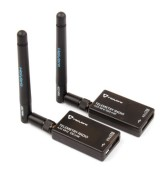
\includegraphics[scale=0.3]{C:/Users/ACER/Downloads/Template-LaTeX-Tugas-Akhir-Sarjana-Terapan-UNY-main/gambar/6}
	\caption{Throttle}
	\label{fig:6}
\end{figure}

\subsection{Pitch}
Gerakan yang dilakukan drone untuk maju dan mundur di sebut \textit{pitch}, dapat dilakukan dengan gerakan 2 motor bagian belakang bergerak cepat agar menghasilkan daya dorong maju dan 2 motor pada bagian depan bergerak normal, untuk dapat melakukan gerakan mundur 2 motor pada bagian depan berputar cepat sedangkan 2 motor bagian belakang bergerak normal\cite{quan2020multicopter}.Hal tersebut di tunjukan pada \cref{fig:09pitch-300x300}

\begin{figure}[H]
	\centering
	\includegraphics[scale=0.5]{C:/Users/ACER/Downloads/Template-LaTeX-Tugas-Akhir-Sarjana-Terapan-UNY-main/gambar/09_pitch-300x300}
	\caption{Pitch}
	\label{fig:09pitch-300x300}
\end{figure}

\subsection{Yaw}
Gerakan \textit{yaw} pada drone untuk berputar searah dan berlawanan dengan jarum jam, untuk putaran berlawanan dengan jarum jam konfigurasi motor depan sebelah kanan dan motor belakang sebelah kiri bergerak cepat, kemudian untuk putaran searah jarum jam dapat dilakukan sebaliknya\cite{quan2020multicopter}.Hal tersebut di tunjukan pada \cref{fig:5}

\begin{figure}[H]
	\centering
	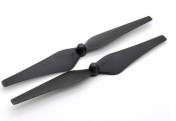
\includegraphics[scale=0.3]{C:/Users/ACER/Downloads/Template-LaTeX-Tugas-Akhir-Sarjana-Terapan-UNY-main/gambar/5}
	\caption{Yaw}
	\label{fig:5}
\end{figure}


\subsection{Roll}
Gerakan manuver kanan dan ke kiri disebut \textit{roll}, untuk melakukan gerakan manuver baik kanan dan kiri, terdapat konfigurasi putaran motor, manuver kanan konfigurasi dari putaran 2 motor bagian kiri secara cepat dan 2 motor bagian kanan bergerak normal dan untuk melakukan manuver kiri sebaliknya\cite{quan2020multicopter}.Hal tersebut di tunjukan pada \cref{fig:10roll-300x300}

\begin{figure}[H]
	\centering
	\includegraphics[scale=0.5]{C:/Users/ACER/Downloads/Template-LaTeX-Tugas-Akhir-Sarjana-Terapan-UNY-main/gambar/10_roll-300x300}
	\caption{Roll}
	\label{fig:10roll-300x300}
\end{figure}

\section{Open CV}
Open Computer Vision, merupakan sebuah library gratis yang digunakan untuk melakukan \textit{image processing} yang dikembangkan oleh Intel Corporation. Bertujuan agar komputer mempunyai kemampuan yang mirip dengan cara pengelohan visual pada manusia. Modul pustaka OpenCV ini dibangun dengan fleksibel untuk menyelesaikan sebagian besar masalah computer vision yang solusinya memang telah tersedia, seperti memotong citra \textit{(cropping)}, meningkatkan kualitas citra dengan memodifikasi kecerahan, ketajaman, kontras, deteksi benuk, segmentasi citra, deteksi objek yang bergerak serta mengenali objek seperti \textit{landing pad}\cite{ratna2020pengolahan}.

\section{Computer Vision}
\textit{Computer Vision} adalah cabang dari kecerdasan buatan serta ilmu komputer yang fokus pada pengembangan algoritma serta teknik guna memungkinkan komputer memperoleh, memproses, serta memahami informasi visual di dunia nyata\cite{dipura2024teknologi}. \textit{Computer Vision} kini telah meluas ke berbagai bidang mulai dari perekaman hingga data mentah hasil ekstrasi pola gambar serta interpretasi informasi. Ini memiliki konsep, teknik, serta ide dari proses gambar digital, pengenalan pola, kecerdasan buatan dan grafis komputer. Sebagian besar tugas dalam \textit{Computer Vision} berkaitan dengan proses memperoleh informasi mengenai peristiwa ataupun deskripsi. Visi pada komputer adalah kombinasi pemrosessan gambar serta pengenalan pola gambar. \textit{Output} dari proses tersebut ialah \textit{Computer Vision} paham akan gambar yang telah di \textit{input} sebelumnya. Pengembangan bidang ini dilakukan dengan adaptasi kemampuan penglihatan manusia saat mengambil informasi yang berada dihadapanya.  Computer Vision berkembang serta bergantung pada sistem teknologi komputer, baik tentang peningkatan kualitas gambar maupun pengenalan gambar. Berikut contoh \textit{Computer Vision} yang ada:

\subsection{Object Detection}
Tugas deteksi objek mengenali atau menentukan beberapa objek dalam sebuah gambar, kaitkan label dengan masing masing objek. keluaran deteksi objek berupa label kelas dan kotak pembatas pada setiap gambar. Sasaranya dengan mengidentifikasikan objek dan menentukan lokasi pada gambar. Contoh kasus dari objek deteksi menerbangan secara otonom. Hal tersebut di tunjukan pada \cref{fig:12}

\begin{figure}[H]
	\centering
	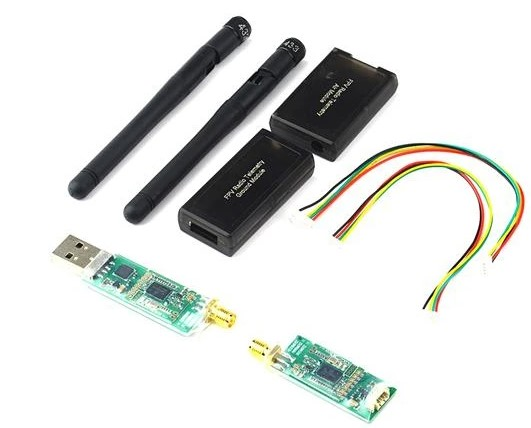
\includegraphics[scale=0.5]{C:/Users/ACER/Downloads/Template-LaTeX-Tugas-Akhir-Sarjana-Terapan-UNY-main/gambar/12}
	\caption{Object Detection}
	\label{fig:12}
\end{figure}

\subsection{Image Processing}
Pengolahan citra (image processing) adalah teknik mengolah citra yang mentransformasikan citra masukan menjadi citra lain agar keluaranya memiliki kualitas yang lebih baik dibandingkan kualitas citra masukan sebelumnya\cite{jauharin2015pengolahan}. Pengolahan citra sangat bermanfaat, diantara manfaat itu ialah untuk meningkatkan kualitas citra, mengidentifikasi objek, menghilangkan cacat pada citra, penggabungan dengan bagian citra yang lain. Dengan memanfaatkan teknologi tersebut, maka diharapkan adanya suatu aplikasi yang dapat menangkap suatu obyek yang ada di depan kamera bisa mengidentifikasi jenis objek serta mentracking objek yang dilakukan secara realtime. Dengan menggunakan webcam yang disambungkan ke PC (Personal Komputer) untuk menangkap gambar secara \textit{real time}, kemudian gambar diolah menggunakan metode template matching berbasis \textit{image processing}, dengan cara membandingkan image database yang telah dibuat dengan pengambilan gambar secara \textit{real time}. sehingga komputer dapat mengidentifikasi dan melakukan tracking objek tersebut. Apabila cocok dengan database, maka output yang dihasilkan berupa suara yang sesuai dengan gambar objek. Hal tersebut di tunjukan pada \cref{fig:im}

\begin{figure}[H]
	\centering
	\includegraphics[scale=0.3]{C:/Users/ACER/Downloads/Template-LaTeX-Tugas-Akhir-Sarjana-Terapan-UNY-main/gambar/im}
	\caption{Image Processing}
	\label{fig:im}
\end{figure}


\section{PID Controller}
Kendali PID merupakan pengendali pada sistem umpan balik yang banyak digunakan pada sistem kontrol secara umum dan dalam skala besar. Kontroler berupaya untuk meminimalkan dan mengecilkan nilai pada keluaran dengan mengatur dan menyesuaikan input proses \textit{control}. Kendali PID terdiri dari tiga buah parameter konstan yang terpisah yaitu Proportional, Integral dan Derivative. Dari ketiga parameter tersebut dapat dinotasikan dengan P, I dan D\cite{leal2021design}. Nilai proportional (P) menentukan nilai kesalahan pada saat ini, nilai integral (I) menghitung nilai kesalahan dari sebelumnya, dan nilai derivative (D) memprediksi nilai kesalahan yang akan terjadi. Jumlah kesetimbangan dari ketiga parameter tersebut dapat digunakan untuk mengatur dan mengontrol suatu sistem  \textit{(plant)} menjadi hasil keluaran respon sesuai yang diinginkan. Hal tersebut di tunjukan pada \cref{fig:pid}

\begin{figure}[H]
	\centering
	\includegraphics[scale=0.5]{C:/Users/ACER/Downloads/Template-LaTeX-Tugas-Akhir-Sarjana-Terapan-UNY-main/gambar/pid}
	\caption{PID Controller}
	\label{fig:pid}
\end{figure}

\section{Python}
Python adalah satu bahasa pemograman tingkat tinggi bersifat interpreter, intrafktif, \textit{object-oriented} dan dapat beroprasi pada semua platfrom seperti Linux, Windows, Mac, dan platfrom lainnya. Python adalah salah satu bahasa pemrograman tingkat tinggi yang mudah untuk dipelajari karena sintaks yang jelas, yang dikombinasikan dengan penggunaan modul-modul yang mempunyai struktur data tingkat tinggi, serta siap untuk digunakan. \textit{Source code} aplikasi phyton biasanya akan dikompilasi menjadi format perantara yang dikenal dengan \textit{byte code} yang kemudian akan di eksekusi\cite{ratna2020pengolahan}.


\section{Mission Planner}
Mission Planner adalah produk dari ardupilot, software yang diciptakanoleh Michael Osborn dan tim pengembanganya yang di kasih nama \textit{ardupilot}, ini digunakan sebagai GCS untuk pesawat dan \textit{quadcopter} yang menggunakan \textit{frimware} dari \textit{ardupilot}\cite{kurniawan2022pengembangan}.Hal tersebut di tunjukan pada \cref{fig:d}

\begin{figure}[H]
	\centering
	\includegraphics[scale=0.9]{C:/Users/ACER/Downloads/Template-LaTeX-Tugas-Akhir-Sarjana-Terapan-UNY-main/gambar/d}
	\caption{Mission Planner}
	\label{fig:d}
\end{figure}

Mision planner dikembangkan secara khusus untuk merencanakan \textit{autonomous flight}, menjalankan misi tertentu dan juga digunakan untuk pemetaan. Dengan demikian perhitungan manual pengenai ketinggian, kecepatan, skala, dan lainnya dapat di otomasikan. Sebelum quadcopter di terbangkan harus di konfigurasi secara menyeluruh mulai dari penggunaaan parameter yang cocok untuk sebuah misi, pengaturan PID, kaibrasi pengontrol kecepatan elektronik, koneksi antara r\textit{emote control} dengan \textit{quadcopter} serta kalibrasi kompas.